\chapter{隐藏需求对话挖掘方法的验证与应用}
本章目的在于介绍数据集设置、通过把FRMiner与近年先进的需求识别基准方法和常见文本分类模型的效果对比验证孪生网络在复杂对话分类中的有效性、对模型参数即数据增强倍数进行定量分析以及FRMiner在项目间泛化能力实验中的表现,并分别介绍了以上实验的设置和实验结果说明以及基本分析。最后,本章对实现的{\tool}工具的离线、在线训练使用进行介绍说明。

\section{实验数据集设置}
\subsection{数据爬取}
本文的数据是通过Scrapy \footnote{https://scrapy.org/}爬取的。Scrapy是用Python实现的一个为了爬取网站数据、提取结构性数据而编写的应用框架。Scrapy常应用在包括数据挖掘,信息处理或存储历史数据等一系列的程序中。通常用户可以很简单的通过Scrapy框架实现一个爬虫,抓取指定网站的内容或图片。如图\ref{fig:scrapy}所示,Scrapy主要有以下组件构成:Scrapy Engine,Scheduler,Downloader,Spiders,Item Pipeline,Downloader middlewares,Spider middlewares。
\begin{figure}[htbp]
    \centering
    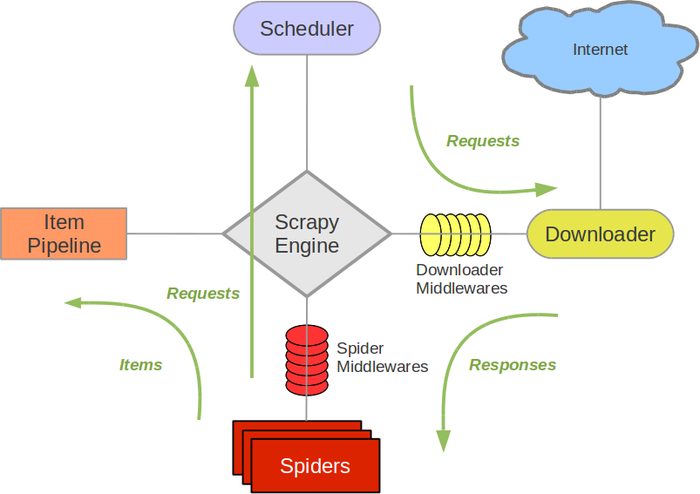
\includegraphics[width=0.6\textwidth]{Img/scrapy.png}
    \bicaption{Scrapy架构图}{The architecture of Scrapy}
    \label{fig:scrapy}
\end{figure}
Scrapy中需要用户自定义的一个核心的组件为Item,其存储了待爬取的对象结构信息。图\ref{fig:echelog}所示为AngularJS项目的IRC记录的格式与内容。
\begin{figure}[htbp]
    \centering
    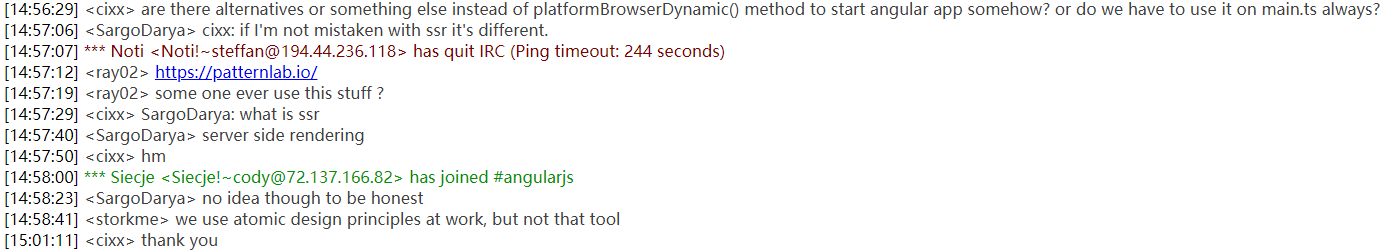
\includegraphics[width=\textwidth]{Img/echelog.png}
    \bicaption{AngularJS项目IRC记录样例}{An example of AngularJS IRC channel}
    \label{fig:echelog}
\end{figure}
因此针对IRC数据,本工作爬取的Item对象的主要结构信息有:Timestamp,UserName和Message。

实验中爬取的对象主要三个开源项目:AngularJS \footnote{https://angularjs.org/},Bootstrap  \footnote{https://getbootstrap.com/}和 Chromium \footnote{https://www.chromium.org/}. 本文选取这三个项目主要有以下几个原因:首先,它们是最近非常活跃的项目;另外这些项目中存在着较大的开源社区;这些项目中的开发者也非常活跃地使用在线聊天进行分享观点、有趣的见解以及讨论哪些功能需要在以后进行实现。例如,在过去的三年里,AngularJS社区里每周平均有2,823条对话。另外,这些历史对话在IRC Archive网站\footnote{https://echelog.com/}中进行存档并允许开放访问,其为本文的工作提供了丰富的语料资源。

\subsection{对话预处理}
本工作首先对爬取到的文本中的非ASCII字符如emojis等转换成ASCII字符串。由于一些低频的Tokens,如URL、邮件地址、代码片段、HTML标签、版本号等对最后的分类结果不会产生帮助,因此对其分别使用\textit{<URL>,<EMAIL>,<HTML>,<CODE>,<ID>}等特殊Tokens进行替换。然后,本工作使用Spacy \footnote{https://spacy.io/},一个优秀的包含分词、词性标注、词干还原等NLP处理功能的工具把句子进行分句、分词。为了减少词语形态学的影响,本研究也使用Spacy对单词进行词干还原和小写转换。

对对话数据进行基本的预处理之后,本文使用JK Kummerfeld等人\cite{kummerfeld2018large}发布的在其标注数据上训练的模型对本文爬取的数据进行对话解耦,在经过人工审核之后,解耦之后的对话质量、可读性以及解耦的准确性较高,达到了可用标准。
对对话进行解耦之后,获取了大量的聊天对话。为了接下来进行数据标注的可行性,并且保证整个对话数据集的整体分布,本研究从这三个项目中分别随机采样了400个对话。然后从中过滤掉以下一些质量较低的对话:
\begin{enumerate}
    \item 使用非英语文本的对话
    \item 包含大量代码和Stack Traces信息的对话
    \item 存在大量拼写错误和语法错误的低质量对话
    \item 包含Channel Robots的对话。
\end{enumerate}

\subsection{数据标注}
标注的对话可以作为本文评估效果的数据集,为了保证标注结果的正确性,本工作建立了一个标注小组,其由两名资深研究人员和四名博士生组成。他们都具有较高的英语水平,并且在软件开发方面做过深入的研究工作,或者为开源项目做出了积极的贡献。本工作将团队分为两组,每个小组由一名负责人(高级研究员)和两名成员组成。每个负责人培训了相应成员如何标注标签并为成员提供咨询。成员对标签的标注结果由负责人进行审查,而每组负责人的结果由其他负责人进行审查。仅当对话在各小组之间的标注达成完全一致时,本研究才接受此对话并将对话以及其标签加入到本文的数据集中。而当对话被标注为不同的标记结果时,将与所有六个人进行讨论,然后通过投票决定最终标签。表\ref{tab:dataset}为爬取到的所有数据集和本文标注的数据集的统计情况。本研究总共从三个开源项目中收集了65,428个对话,并花了720人/小时的时间来标注1,035个对话(总体数据集的1.6%)。

\begin{table}[htbp]
\bicaption{标注对话的统计详情}{The statistic of labeled dialogues}
    \label{tab:dataset}
    \centering
    \footnotesize% fontsize
    \setlength{\tabcolsep}{4pt}% column separation
    \renewcommand{\arraystretch}{1.2}%row space 
\begin{tabular}{|c|c|c|c|c|c|c|}
\hline
\multirow{}{}{} & \multicolumn{3}{c|}{全部聊天记录数据}    & \multicolumn{3}{c|}{抽取样本} \\ \cline{2-7} 
                  & 时间区间          & 对话数   & 句子数    & 对话数    & 句子数     & 需求数  \\ \hline
AngularJS         & 2016.5-2019.4 & 38266 & 406553 & 316    & 9220    & 36     \\ \hline
Bootstrap         & 2014.7-2019.5 & 10358 & 58871  & 379    & 2371    & 76     \\ \hline
Chromium          & 2015.5-2019.7 & 16804 & 118890 & 340    & 4465    & 27     \\ \hline
\multicolumn{2}{|c|}{总计}          & 65428 & 584314 & 1035   & 16056   & 139    \\ \hline
\end{tabular}
\end{table}

\section{验证实验设置}
本部分主要介绍下文中设计的三个实验的基本设置。这三个实验都在三个开源项目数据集上使用了三折交叉验证\cite{DBLP:conf/ijcai/Kohavi95}。首先,本研究将数据集分成三部分,并使用其中两份作为训练集,剩下的一份作为测试集,然后重复这个过程三次,并且每次使用剩下的不同部分作为测试集。在三个实验中,均使用相同的分割数据集。另外,实验环境为Ubuntu操作系统,硬件配置为Intel core i7 CPU,16G RAM,NVIDIA 1060 GPU。


\section{FRMiner进行需求挖掘的有效性实验}
\subsection{实验目的及实验设计}
为了验证{\tool}的有效性,本文基于三个开源项目的聊天记录,对于隐藏需求对话识别实验进行了三折交叉验证。并且针对两个近年效果先进的句子级别的需求发现方法以及四个广泛使用的文本分类方法,本文与其比较了分类表现,以验证FRMiner在有限标注数据上进行自动需求对话识别的有效性。

\textbf{1)基于句子级别需求发现的基线方法}

上文介绍了近年软件工程领域在需求识别方面的研究工作,其中章节2.1中的CNN-based Classifier(CNC)\cite{Huang2018Automating}和Feature Request Analyser(FRA) \cite{shi2017understanding}在需求分类上达到较好的效果。由于原分类器的分类目标是句子,需要将其调整为对话级别的分类器,也即对话中包含为分类器预测为需求意图的句子时,本文认为该对话为需求对话。本文选用这两个方法作为需求分类方面的基线方法,并使用了对应文献中中提供的代码和模型。

CNC是目前从在线问题报告的评论中进行句子分类的最优模型,其使用基于卷积神经网络的方法把句子分为七个类别:信息提供、信息寻找、提出需求、问题提出、问题发现、方面验证和无意义的语句。本文使用其中预测为需求的类别,即将包含需求句子的对话分类为需求对话。

FRA是一个从在线问题追踪系统中把句子进行需求分类的最优的基于规则的模型,其使用81个规则将句子分为六个类别,本研究将包含类别\textit{Intent}的句子的对话分类为需求对话,同时,不包含\textit{Intent}句子的对话为非需求对话。

\textbf{2)基于文本分类的基线方法}

对于四个基于机器学习的文本分类方法,本文选用如章节2.3中所述的朴素贝叶斯(NB)\cite{mccallum1998comparison}、随机森林(RF)\cite{liaw2002classification}、梯度提升决策树(GBDT)\cite{ke2017lightgbm} 和FastText(FT)\cite{joulin2016bag} 作为基线方法。

NB为一个简单的使用词袋模型和贝叶斯规则的文本分类模型,它通过先验概率和学习训练数据得到的条件概率得到句子的后验概率,也即,给定一个句子,它可以推断出句子在所有类别下的概率。
RF是一个使用多个树构建的集成机器学习模型,每个树都为最后的分类结果做贡献。在训练RF时,本研究设置树的最大深度为2。
GBDT是另一个集成学习方法,和RF的不同在于它的树是通过前面树的残差来决定的。当训练GBDT时,本文设置初始学习率为1.0,树的最大深度为1。
FT是基于一个结构上类似于word2vec的浅层神经网络的文本分类方法,本文在实验中训练100轮,并设置初始学习率为1.0,输入n-gram的窗口大小为2。

对于四个文本分类模型,本文使用官方提供的包 \footnote{https://scikit-learn.org/stable/} \footnote{https://fasttext.cc/},并且提取了词频-逆文档频率(TFIDF)\cite{joachims1996probabilistic}作为对话特征向量来进行对话文本分类。
% 探索如何基于稀疏或者稠密向量高效表示句子语义、语法信息是自然语言处理研究人员关注的一项工作。
TF-IDF(term frequency–inverse document frequency)常用于信息检索与数据挖掘的加权技术,通过以词频、逆文档频率表示的词的重要性程度来表示句子。TF-IDF主要包含两部分:词频TF和逆文档频率IDF。其中,TF是词在文本中出现的次数,出现次数越多,表示该词越重要并在文本中占据重要的语义。对于词$t_i$来说其TF为,$tf_{i,j}=\frac{n_{i,j}}{\sum_k{n_{k,j}}}$,其中$n_{i,j}$代表该词在文档$d_j$中出现的次数,分母为在文档$d_j$中所有词出现的次数总和。
IDF是词出现在不同文档数的逆,词出现的次数越多,代表该词属于停用词如“的”、“是”、“了”等的概率越大。对于一个此来说,其IDF为$idf_{i}=\frac{|D|}{\{j:t_i \in d_j\}}$,其中$|D|$为文档总数,$\{j:t_i \in d_j\}$代表包含词$t_i$的文档总数,如果该词语不在语料库中,就会导致被除数为零,因此一般情况下使用$1+\{j:t_i \in d_j\}$。当有TF和IDF后,将这两个值相乘,也即$tfidf_{i,j}=tf_{i,j}\times idf_i$,就能得到一个词在文档集中的TF-IDF的值。在得到每个词的TFIDF后,对于文档集的词集合$V$,通常使用长度为$|V|$的向量表示文档,其中每个元素的值为出现在该文档的词的TFIDF值,没有出现则对应位置为零。然后可以得到文档的向量化表示,继而作为句子的文本向量表示运用到基线方法中。


针对模型参数优化,本文使用网格搜索来微调四个文本分类模型的参数,使其达到最优效果。
另外,在以上的基线模型中,本文均使用了随机上采样\cite{ling1998data}来解决数据集的类别不均衡问题。

\subsection{实验结果及分析}
表格\ref{tab:rq1}展示了每个项目三折交叉验证中不同方法达到的不同效果。
\begin{table}[htb]
\bicaption{每个项目在项目内通过不同方法取得的效果}{The performance achieved by different approaches for each project in intra-project validation}
    \label{tab:rq1}
    \centering
    \footnotesize% fontsize
    \setlength{\tabcolsep}{4pt}% column separation
    \renewcommand{\arraystretch}{1.2}%row space 
\begin{tabular}{|c|c|c|c|c|c|c|c|c|c|c|}
\hline
\multicolumn{2}{|c|}{\multirow{2}{*}{\diagbox{方法\qquad}{效果\qquad}}}   & \multicolumn{3}{c|}{AngularJS}                           & \multicolumn{3}{c|}{Bootstrap}                         & \multicolumn{3}{c|}{Chromium}                          \\ \cline{3-11} 
\multicolumn{2}{|c|}{}                           & Precision        & Recall           & F1               & Precision        & Recall           & F1               & Precision        & Recall           & F1               \\ \hline
\multirow{2}{*}{本文方法}        & FRMiner   & \textbf{90.28\%} & \textbf{89.73\%} & \textbf{90.00\%} & \textbf{86.28\%} & \textbf{88.78\%} & \textbf{87.52\%} & \textbf{89.00\%} & \textbf{87.00\%} & \textbf{88.00\%} \\ \cline{2-11} 
                                     & p-FRMiner & 31.71\%          & 54.17\%          & 40.00\%          & 50.00\%          & 47.80\%          & 48.98\%          & 14.00\%          & 44.00\%          & 20.00\%          \\ \hline
\multirow{2}{*}{已有研究方法}    & CNC       & 7.70\%           & 44.44\%          & 13.13\%          & 16.38\%          & 34.21\%          & 22.13\%          & 9.56\%           & 67.00\%          & 16.73\%          \\ \cline{2-11} 
                                     & FRA       & 13.67\%          & 80.33\%          & 23.35\%          & 23.00\%          & 48.67\%          & 31.00\%          & 12.00\%          & {81.00\%} & 20.00\%          \\ \hline
\multirow{4}{*}{文本分类方法} & NB        & 20.00\%          & 27.67\%          & 22.33\%          & 25.67\%          & {62.00\%} & 36.00\%          & 14.33\%          & 44.33\%          & 21.00\%          \\ \cline{2-11} 
                                     & GBDT      & 36.00\%          & 22.33\%          & 27.33\%          & 41.67\%          & 35.67\%          & 38.33\%          & 9.33\%           & 7.33\%           & 8.00\%           \\ \cline{2-11} 
                                     & RF        & 52.67\%          & 11.00\%          & 16.33\%          & 57.00\%          & 29.00\%          & 38.33\%          & 0.00\%           & 0.00\%           & NA               \\ \cline{2-11} 
                                     & FT        & 23.33\%          & 5.33\%           & 8.67\%           & 57.67\%          & 29.00\%          & 38.33\%          & 38.00\%          & 9.10\%           & 15.00\%          \\ \hline
\end{tabular}
\end{table}

其中,对于Precision、Recall、F1值最优的结果使用黑体标出。可以看到,{\tool}在三个项目中均取得了最好的效果,平均精确度、召回率、F1值分别是88.52\%, 88.50\%, and 88.51\%。另外,p-{\tool}比所有的基线方法效果要好,表明了通过BiLSTM记忆上下文信息可以帮助从聊天记录中进行隐藏需求对话识别的文本分类任务。

对于两个句子级别的分类方法,CNN仅能取得17.33\%的平均F1值,主要是因为CNC是在问题评论语料库上而不是需求对话训练得到的。然而,其依然能取得48.55\%的平均召回率,这表明在这两个领域里面应该存在着共有的分类相关模式。同时,基于规则的分类器FRA可以在六个基线方法中取得最高的平均召回率,其为70.00\%,并且在AngularJS和Chromium两个项目上分别可以取得80.33\%和81.00\%的召回率。虽然其精确度较低,但是由于FRA的高召回率,其预测结果包含大量真正的需求对话,这也意味着对话信息中的需求的句子也服从FRA的规则。另一方面,由于FRA使用基于规则的分类方法,而不是有监督的机器学习方法,FRA在挖掘大规模的聊天信息方面更加高效,并且,基于FRA较高的召回率这一优势,本文可以通过其进行标注数据初期的粗粒度召回。

对于四个文本分类方法,NB在其中取得了最好的效果。虽然RF在四个方法里面取得最高的F1值-27.33\%,但其在Chromium项目上存在着欠拟合问题,即不能很好的建模训练数据,其原因主要在于Chromium项目数据集不充分,不能得到很好的训练并学习到相关模式。以下是本文提出的{\tool}在效果上大大超过四个传统文本分类模型的原因:
\begin{enumerate}
    \item 和传统的文本分类模型相比,神经网络模型具有更大的信息容量,尤其在建模复杂的对话模型上能取得较好的效果。
    \item 直觉上,模型判断两个对话的类别是否相似要比将每个对话分类为其类别更加容易进行学习。
    \item 由于数据集规模较小,普通的文本分类模型存在在欠拟合问题,而由于{\tool}是一个pair-wise方法,可以将原数据集增广为较大规模,可以保证模型在充足的数据集上进行训练。
\end{enumerate}

总的来说,{\tool}效果上明显超过两个句子级别的需求分类方法和四个传统文本分类方法。由于CNC和FRA两个句子级别基线方法可以直接应用于聊天记录数据并且达到较高的召回率,他们在数据标注方面可以起到粗粒度召回的作用。

\section{孪生网络在FRMiner中的有效性实验}
\subsection{实验目的及实验设计}
为了检验引入孪生网络而带来的效果提升,本文构建了以Single-Instance为输入的基本上下文敏感对话分类模型p-{\tool}和使用Pair-Instance作为输入的{\tool}进行效果对比。之后,本文逐渐增加Pair-Instance训练集的大小来检验模型效果提升和数据集增强的关系。


需要注意的是,p-{\tool}和{\tool}是不同的分类模型,其中,如图\ref{fig:model-cls}所示,p-{\tool}是在前文所述的上下文敏感对话模型{\dm}的基础上添加线性分类层,并接受单个对话作为输入,其可以对需求对话进行分类识别。
\begin{figure}[htbp]
    \centering
    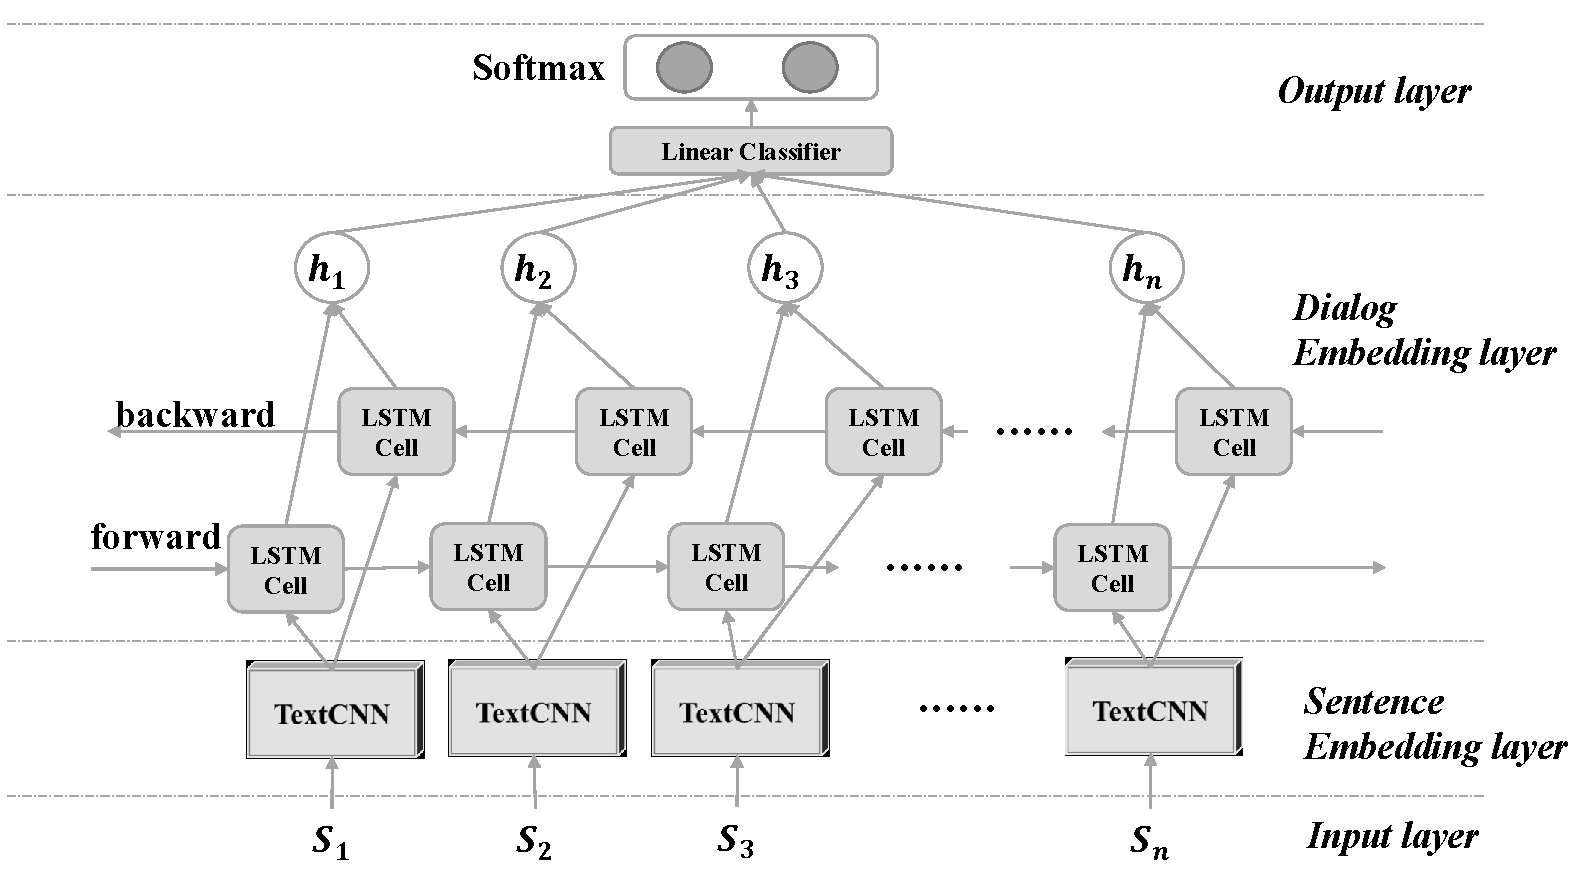
\includegraphics[width=\textwidth]{Img/model_cls.pdf}
    \bicaption{p-{\tool}上下文敏感对话分类模型}{p-{\tool} Context-aware Dialog Classification Model}
    \label{fig:model-cls}
\end{figure}

而{\tool}使用一对对话作为输入,其结构也可以通过修改p-{\tool}的结构得到。具体的,首先,移除p-{\tool}上层的分类层;拼接两个共享参数的相同的p-{\tool};最后,加上线性相似度度量层。

在实验部分,首先,本文使用相同大小的数据集来训练{\tool}和p-{\tool},并观察最后的效果提升。然后,把训练集分别增广到5倍、10倍、20倍和30倍来观察效果变化。因为{\tool}可以利用孪生网络天然的解决数据类别不均衡问题,然而,p-{\tool}不能平衡数据集,因此,本文通过随机上采样来均衡p-{\tool}的数据集。为了保证本文实验的准确性,{\tool}和p-{\tool}使用相同的超参数进行训练,包括每层的维度,网络的深度以及学习率等。


\subsection{实验结果及分析}

图\ref{fig:p-FR}展示了分别在相同数量的Single-Instance和Pair-Instance数据集上训练的p-{\tool}和{\tool}的效果。其中蓝色的条形图代表p-{\tool}的效果,其是在两折数据上训练的结果,训练数据量如图例所示。橙色的条形图代表使用孪生网络的{\tool}的效果,图例所示为Pair-Instance的数量。可以看到,当训练样本量相同时,{\tool}比p-{\tool}取得了明显的较高的分类效果。{\tool}对于精确度、召回率、F1值分别平均提高了46.79\%,31.13\%,42.90\%。

\begin{figure}[htb]
\centering
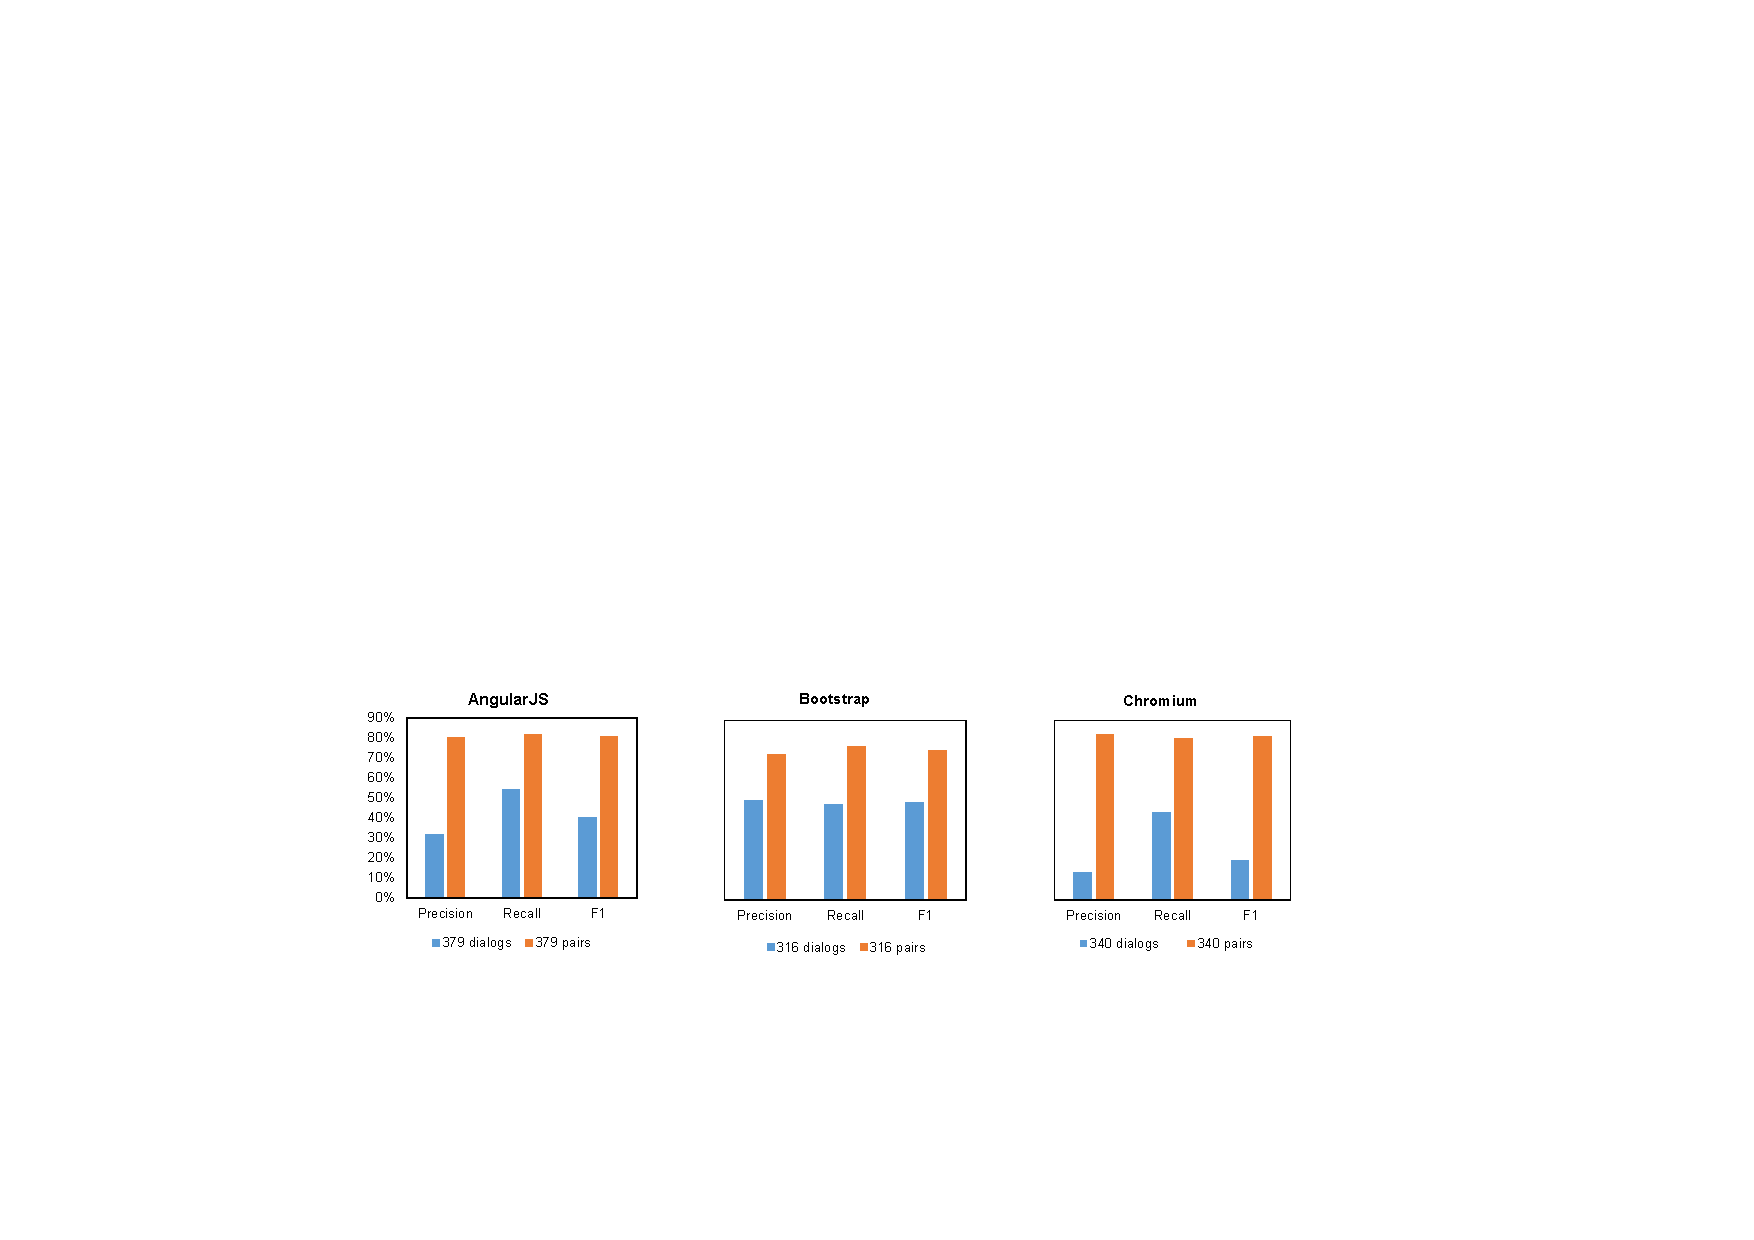
\includegraphics[width=\textwidth]{Img/p-FRvsFR.pdf}
\bicaption{p-FRMiner和FRMiner在相同大小训练集上的表现}{The comparison performances of p-FRMiner and FRMiner with the same volume of original training data}
\label{fig:p-FR}
\end{figure} 

图\ref{fig:FR-size}展示了Pair-Instance训练数据量的增广程度、分类效果的提升和在训练阶段花费的时间成本之间的关系。

\begin{figure}[htb]
\centering
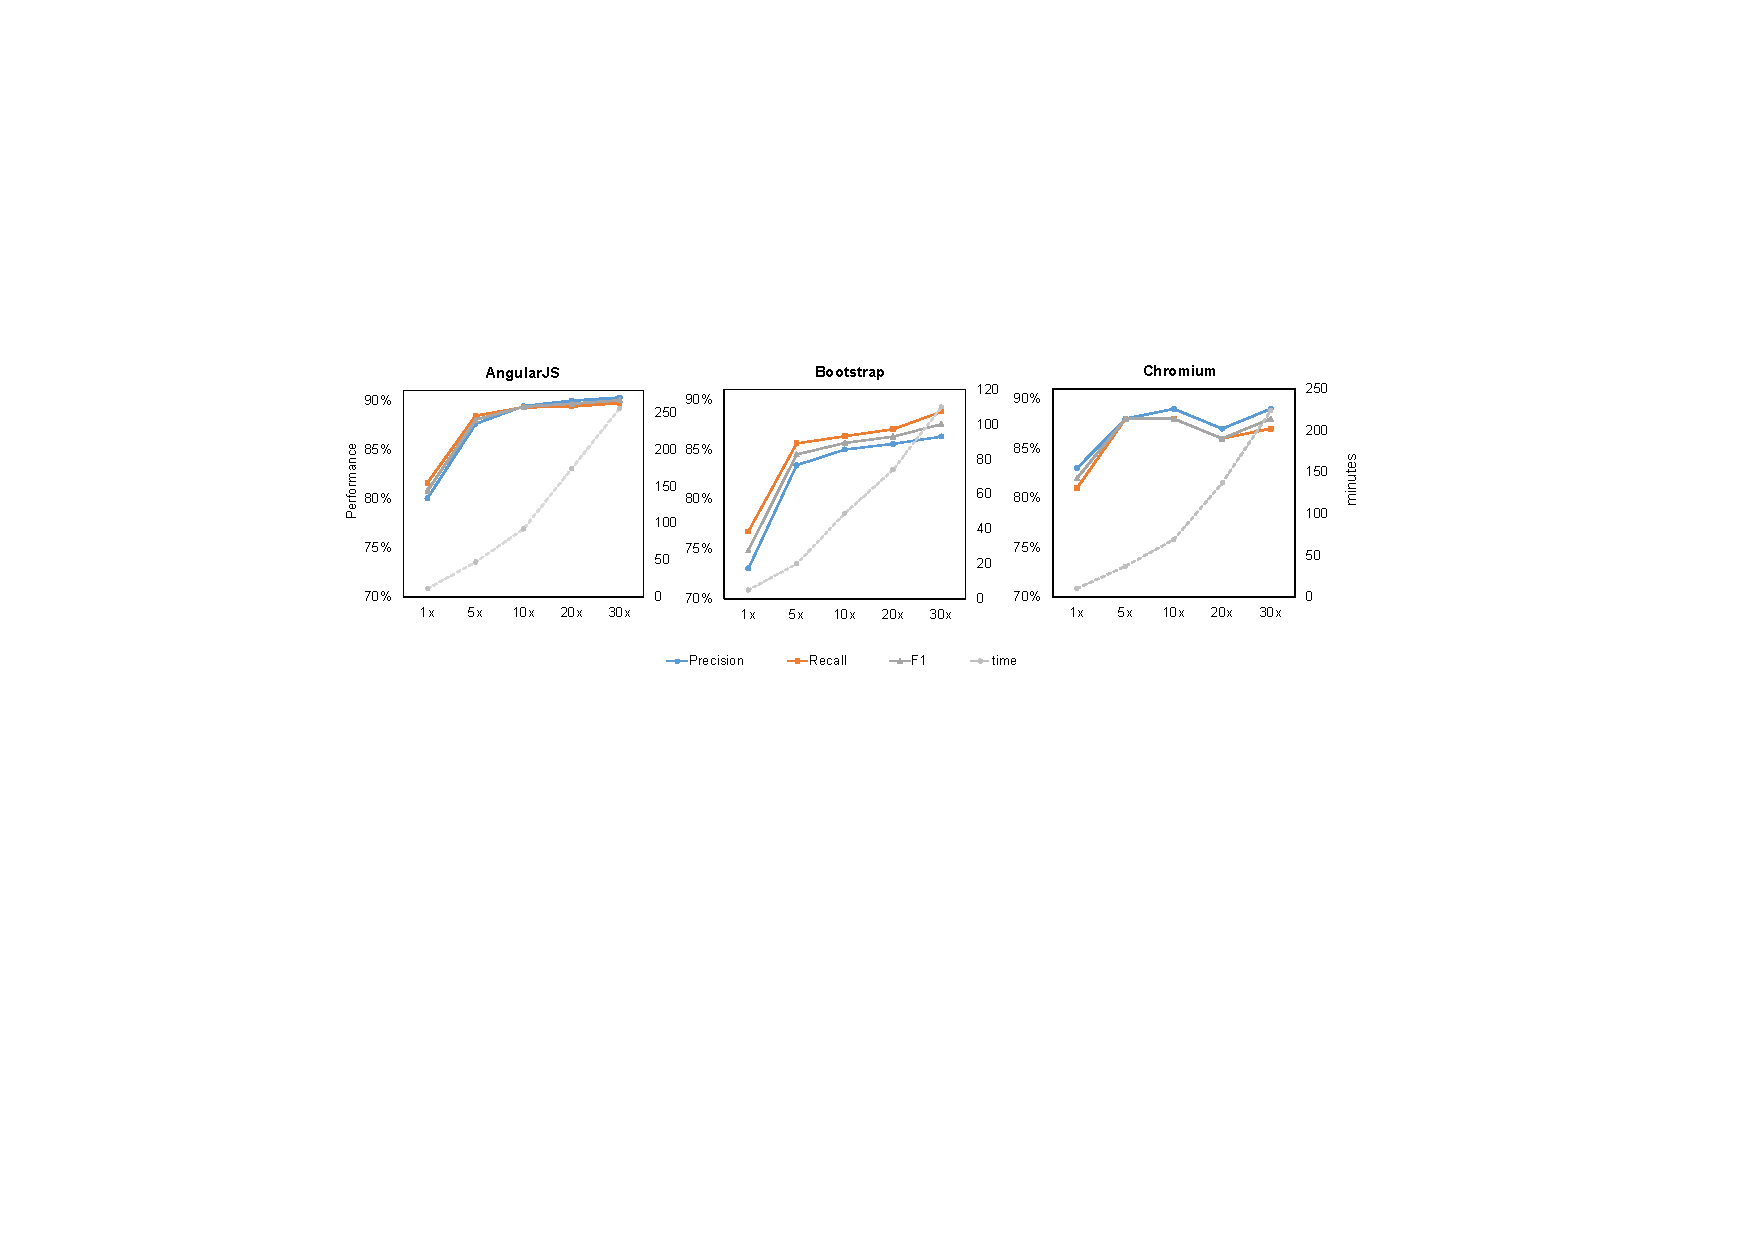
\includegraphics[width=\textwidth]{Img/FRMiner_size.pdf}
\bicaption{FRMiner在不同大小Pair数据集上的表现}{The performances of FRMiner when generating different numbers of pairs}
\label{fig:FR-size}
\end{figure} 

初始训练集数据量(1X数据量)如图\ref{fig:p-FR}所示,分别为379,316和340条数据。可以看到,通过扩大Pair-Instance训练集大小可以提高模型效果。当Pair-Instance训练集大小从1倍增广到30倍后,精确度、召回率、F1值分别平均提高了9.82\%,8.72\%和9\%。观察到模型效果在训练集扩大到5倍时提高最快,而从5倍增广到30倍时,三个项目上的效果提升较小。 当增广到20倍时,在Chromium项目上的效果甚至有较小的下降。而训练阶段所花费的时间基本呈现线性增加的特点。因此,本文认为将训练集增广到5倍是在训练效率和模型效果之间的一个较好的均衡的值。

总结来说,{\tool}比p-{\tool}可以更好地解决对话分类问题,在模型精确度、召回率、F1值上平均提升较大。实验结果表明了在训练数据较少的情况下,分辨两个对话是否同属于需求对话要比对单个对话分类为其类别更加简单。本文在实验中使用了5倍数据增广,因为更大的数据增强增加了模型训练时间成本,同时并不能带来明显更好的模型效果,而5倍数据增广较好的平衡了模型效果和训练时间成本。


\section{FRMiner的项目间泛化能力实验}
\subsection{实验目的及实验设计}
接下来,本文通过在三个开源项目数据集上验证了{\tool}在不同项目领域间的泛化能力。本实验迭代的使用其中两个项目作为训练集,剩下的一个项目作为测试集。为进行泛化能力对比,本实验也在基线方法上进行跨项目验证。其中,实验中所用到的参数和实验5.3中保持一致。


\subsection{实验结果及分析}

表格\ref{tab:rq3}展示了在跨项目实验中每个项目作为测试集的表现。


\begin{table}[!htbp]
\bicaption{每个项目在跨项目实验中使用不同方法达到的效果}{The performance achieved by different approaches for each project in cross-project validation}
\label{tab:rq3}
    \centering
    \footnotesize% fontsize
    \setlength{\tabcolsep}{4pt}% column separation
    \renewcommand{\arraystretch}{1.2}%row space 
\begin{tabular}{|c|c|c|c|c|c|c|c|c|c|c|}
\hline
\multicolumn{2}{|c|}{}                                             & \multicolumn{3}{c|}{AngularJS}                                                                     & \multicolumn{3}{c|}{Bootstrap}                                                                   & \multicolumn{3}{c|}{Chromium}                                                                    \\ \cline{3-11} 
\multicolumn{2}{|c|}{\multirow{-2}{*}{\diagbox{方法\qquad}{效果\qquad}}}                    & Precision                      & Recall                         & F1                             & Precision                      & Recall                         & F1                             & Precision                      & Recall                         & F1                             \\ \hline
                                      & FRMiner                    & \textbf{85.23\%}               & \textbf{86.56\%}               & \textbf{85.89\%}               & \textbf{86.84\%}               & \textbf{85.89\%}               & \textbf{86.37\%}               & \textbf{85.87\%}               & \textbf{86.81\%}               & \textbf{86.34\%}               \\ \cline{2-11} 
\multirow{-2}{*}{本文方法}        & p-FRMiner                  & 31.03\%                        & 50.00\%                        & 38.30\%                        & 27.56\%                        & 69.08\%                        & 39.40\%                        & 16.00\%                        & 50.00\%                        & 24.24\%                        \\ \hline
                                      & {CNC} & {7.70\%}  & {44.44\%} & {13.13\%} & {16.38\%} & {34.21\%} & {22.13\%} & {9.56\%}  & {67.00\%} & {16.73\%} \\ \cline{2-11} 
\multirow{-2}{*}{已有研究方法}    & {FRA} & {13.67\%} & {80.33\%} & {23.35\%} & {23.00\%} & {48.67\%} & {31.00\%} & {12.00\%} & {81.00\%} & {20.00\%} \\ \hline
                                      & NB                         & 16.00\%                        & 75.00\%                        & 26.00\%                        & 27.00\%                        & 36.00\%                        & 31.00\%                        & 7.00\%                         & 26.00\%                        & 12.00\%                        \\ \cline{2-11} 
                                      & GBDT                       & 18.00\%                        & 14.00\%                        & 16.00\%                        & 30.00\%                        & 11.00\%                        & 16.00\%                        & 20.00\%                        & 19.00\%                        & 19.00\%                        \\ \cline{2-11} 
                                      & RF                         & 28.00\%                        & 14.00\%                        & 19.00\%                        & 37.00\%                        & 9.00\%                         & 15.00\%                        & 12.00\%                        & 26.00\%                        & 16.00\%                        \\ \cline{2-11} 
\multirow{-4}{*}{文本分类方法} & FT                         & 32.00\%                        & 19.00\%                        & 24.00\%                        & 43.00\%                        & 13.00\%                        & 20.00\%                        & 19.00\%                        & 11.00\%                        & 14.00\%                        \\ \hline
\end{tabular}
\end{table}

其中,最优的精确度、召回率、F1值使用黑体表示。需要注意的是,因为CNC和FRA是基于各自数据集训练的模型或者提取的规则,其不适用于跨项目实验,因此CNC和FRA的效果和项目内三折交叉实验的结果相同,为了对比和分析,本文将表格\ref{tab:rq1}中的数据复制到表格\ref{tab:rq3}中。可以看到,{\tool}在跨项目实验中表现较好,其F1值仅相比项目内实验平均降低2.27\%。主要原因在于不同项目中表达需求意图的对话存在着共有的模式,并且这些模式可以在项目间进行共享。实验结果表明{\tool}可以学习到需求对话相关的范式,并且可以泛化到其他项目中,同时,这也表明开发者在不同的社区和项目中使用相似的模式表达需求意图。对于p-{\tool},其平均F1值相比项目内实验降低了10.51\%。

对于四个文本分类基线方法,NB取得了最高的F1值-23\%,并且相比项目内实验仅降低了3.44\%。注意到大多文本分类方法在Angular和Chromium两个项目上的模型效果比项目内实验要高,其主要是由于以下原因:
\begin{enumerate}
    \item 交叉项目实验中的训练数据集包含两个项目的数据集,而项目内实验仅包含一个项目的2/3大小的数据集。交叉项目实验可以在更充分的训练数据上进行训练。
    \item 由于交叉项目实验包含两个项目的数据集,更广泛领域的数据集可以引入不同领域的偏置信息帮助分类器提高泛化能力。
\end{enumerate}

因此,{\tool}在未训练数据集上依然能取得较好的效果,这表明{\tool}在不同项目间具有较好的泛化能力。同时,NB是在所有文本分类方法中从聊天记录中挖掘需求对话最好的方法。

\section{{\tool}工具的离线和在线应用}

本文的{\tool}模型代码以及数据已在\href{https://github.com/FRMiner/FRMiner}{https://github.com/FRMiner/FRMiner}开源,并提供有详细代码使用文档,使用者可运行代码对未标注对话进行需求识别或者基于代码做进一步研究。

通过部署应用本文提供的{\tool}工具,使用者不仅可用于离线训练使用,并且可以集成到发布团队的工作流中进行在线使用,从而可以帮助收集群体需求。

\subsection{{\tool}工具离线训练应用}
在获取{\tool}工具代码之后,用户首先需要配置json文件,其关键字段如下:
\begin{lstlisting}[language = json]
"train_data_path": 训练文件路径,
"validation_data_path": 测试文件路径,
"text_field_embedder": 预训练词向量,
"pos_tag_embedding": pos-tag向量,
"optimizer": 优化器,
"num_epochs": 迭代次数,
"cuda_device": GPU训练
\end{lstlisting}
然后通过\textit{allennlp train FRMiner/config.json -s FRMiner/out/ -f --include-package FRMiner}运行本文提供的{\tool}工具实现,用户可以对已标注数据进行训练和结果评估,并将最终训练模型序列化到目标文件夹。
其中,训练过程如图\ref{fig:model-train}所示。

\begin{figure}[htb]
    \centering
    \begin{subfigure}[b]{0.45\textwidth}
      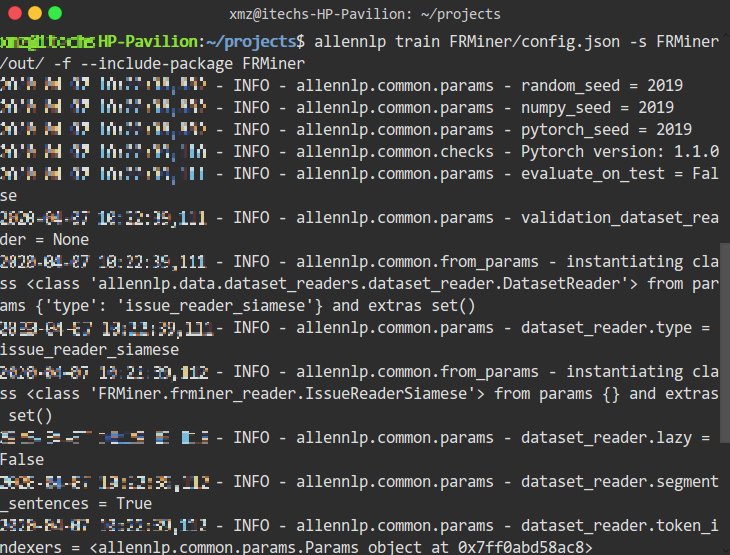
\includegraphics[width=\textwidth]{Img/start.png}
      \caption{}
      \label{fig:start}
    \end{subfigure}%
    ~% add desired spacing
    \begin{subfigure}[b]{0.45\textwidth}
      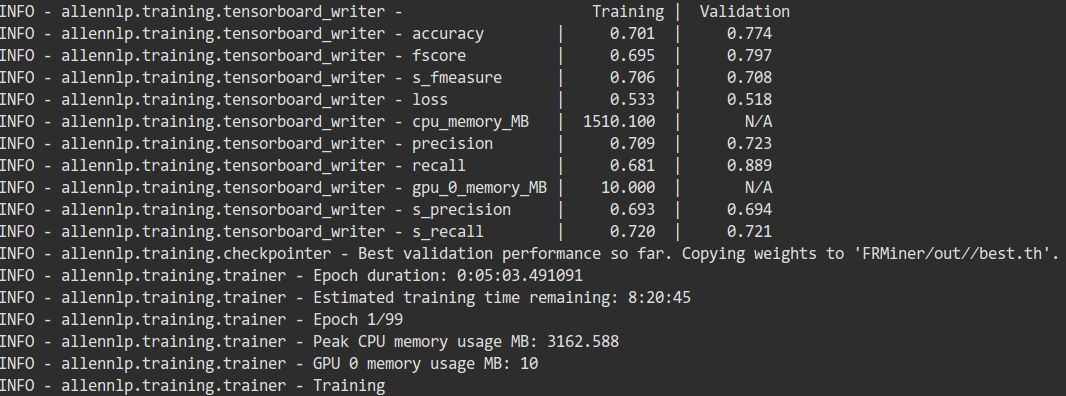
\includegraphics[width=\textwidth]{Img/train.png}
      \caption{}
      \label{fig:train}
    \end{subfigure}
    % ~% line break
    % \begin{subfigure}[b]{0.3\textwidth}
    %   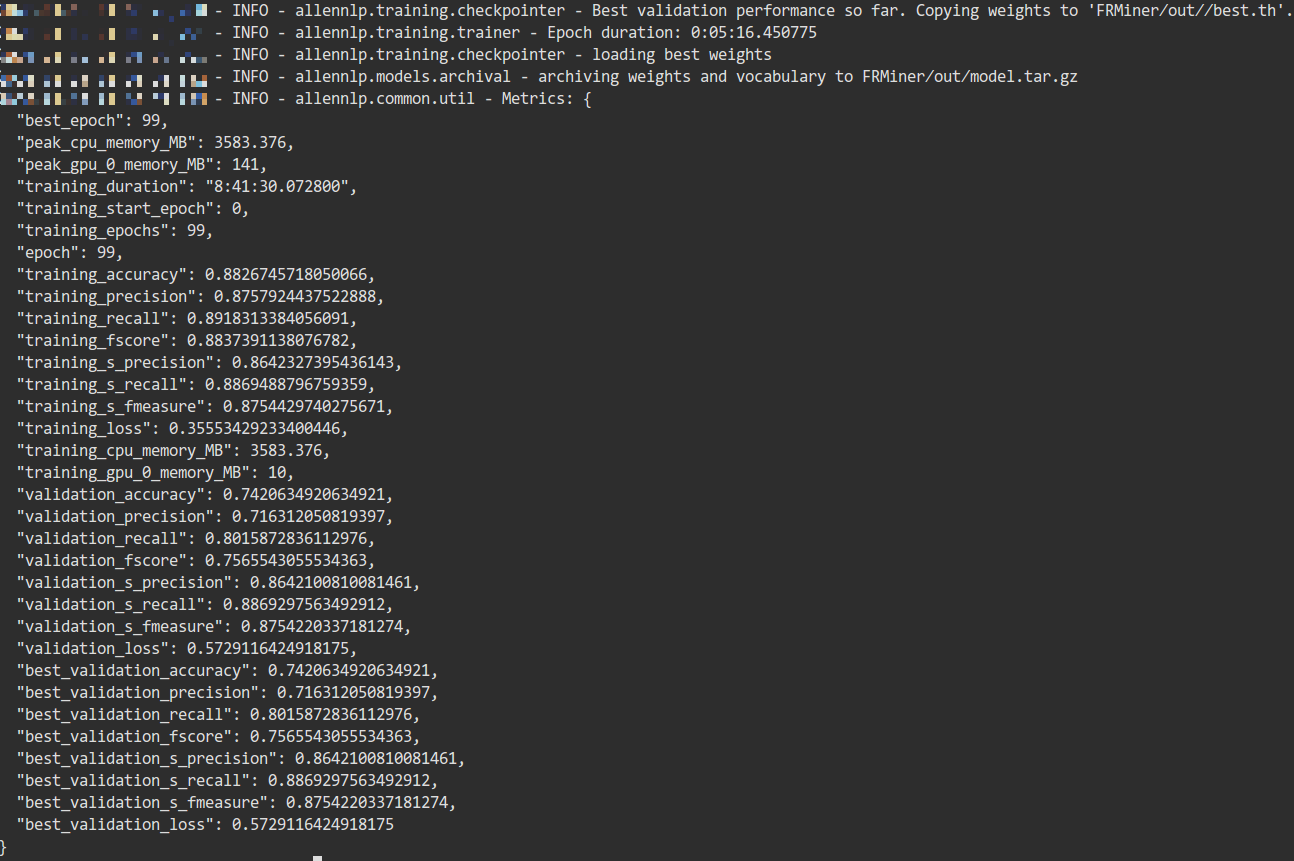
\includegraphics[width=\textwidth]{Img/result.png}
    %   \caption{}
    %   \label{fig:result}
    % \end{subfigure}%
    ~% add desired spacing

    \bicaption{{\tool}训练过程。(a) 为开始训练,(b) 训练过程中的每一轮情况}{The training process of {\tool}. (a) Start training, (b) Details of every epoch during training}
    \label{fig:model-train}
\end{figure}

在经过json配置文件中指定的训练迭代次数后,如图\ref{fig:model-result}所示,{\tool}工具会以json格式输出并保存训练和评估结果。
\begin{figure}[htb]
    \centering
    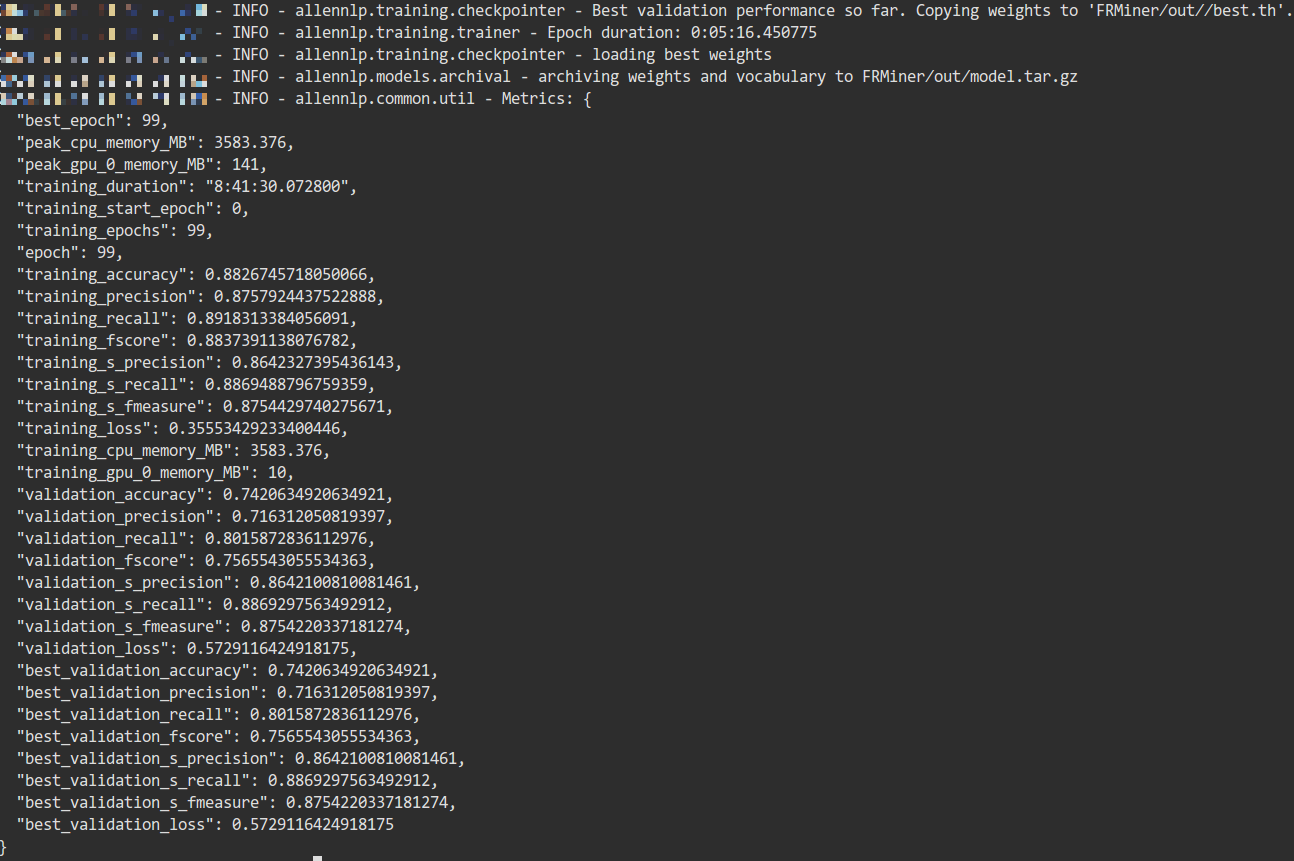
\includegraphics[width=0.8\textwidth]{Img/result.png}
    \bicaption{{\tool}训练和验证结果}{The training and evaluation result of {\tool}}
    \label{fig:model-result}
\end{figure}

在基于本文提供的数据集或者用户自行标注数据集上进行训练之后,用户可以加载训练好的模型,并通过\textit{allennlp predict <模型路径> <未标注对话路径> --output-file=<预测结果存放路径> --predictor=fr\_predictor --include-package=FRMiner},来使用模型对未标注对话进行分类预测。

\subsection{{\tool}工具在线训练应用}
除上文所述的离线使用之外,{\tool}也可以集成部署到如图\ref{fig:workflow}所示的实际工作流场景中进行在线训练使用。
\begin{figure}[htb]
    \centering
    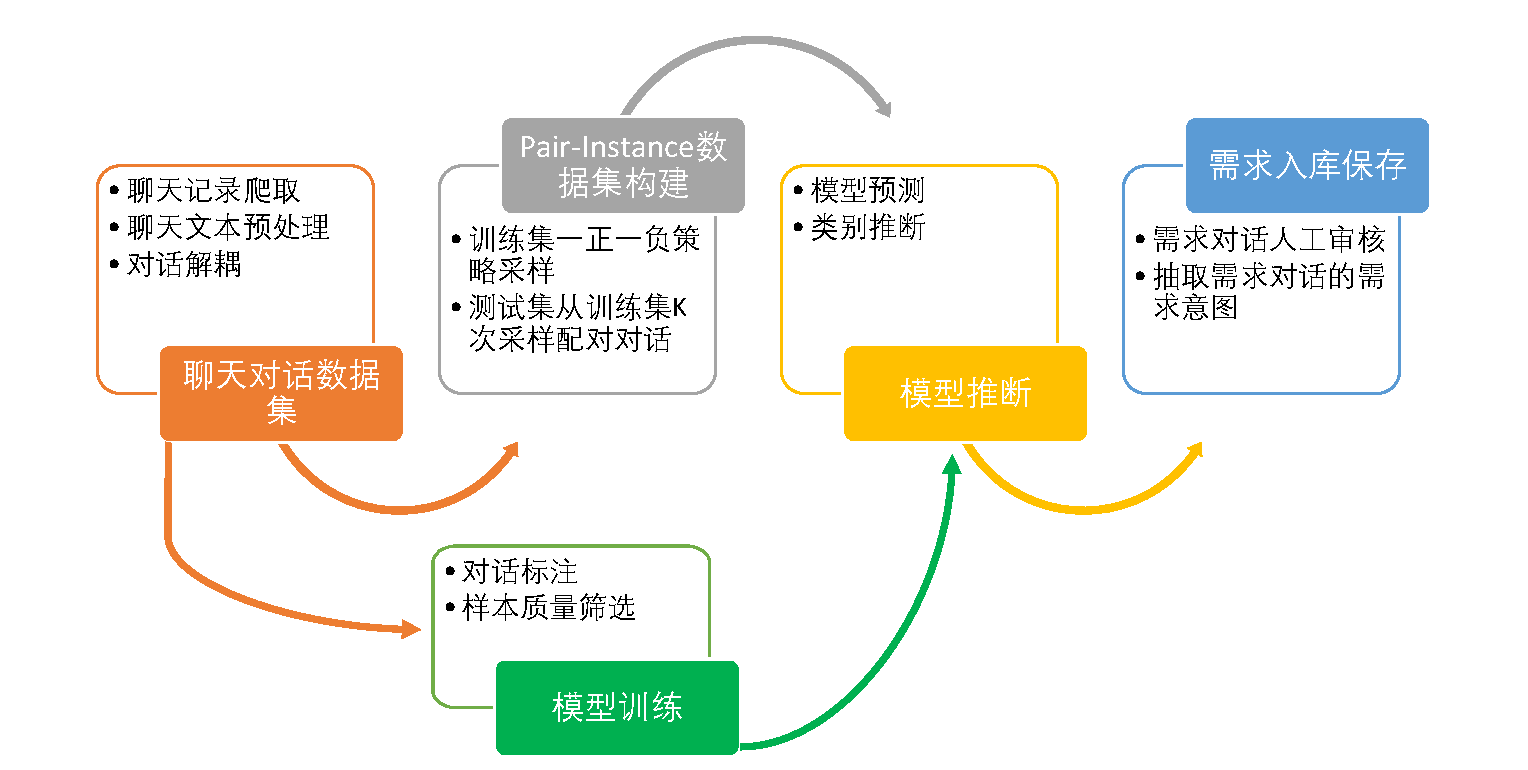
\includegraphics[width=\textwidth]{Img/FRMiner-workflow.pdf}
    \bicaption{FRMiner工作流在线部署}{The online deploy of {\tool} in workflow}
    \label{fig:workflow}
\end{figure}

首先,发布团队需要构建聊天信息监测器或者爬虫来定期从公司的聊天平台收集对话文本信息。然后,使用自动化脚本\cite{kummerfeld2018large}来对原始对话文本进行预处理和对话解耦。接下来,通过前面介绍的对话表示和对话分类过程,{\tool}可以记录所有在表达需求的对话。而发布团队可以使用RSS(Really Simple Syndication)订阅定期监测收集到的隐含的需求对话结果。另外,由于开发者倾向于使用较为一致的方式在对话中表达需求,如“需要在下个版本中实现某功能”、“某功能将会一种解决方法/改进”等,因此仅当数据集的质量或聊天内容发生较大的偏移时{\tool}需要进行重新训练,否则{\tool}不需要经常进行重新训练。

\section{本章小结}

本章首先介绍了实验数据集的获取,接下来主要介绍针对本文提出的{\tool}设计了三个实验,包括{\tool}进行需求识别的有效性实验、孪生网络在{\tool}中的有效性实验以及{\tool}的项目间泛化能力实验的实验设置和参数配置。然后本文针对实验结果进行分析,试验结果表明本文的方法相较于两个句子级别的需求识别方法和四个文本分类方法有较大的性能提升,其中CNC和FRA召回率较高,在四个文本分类方法中NB的效果最好。另外由于开发者在不同项目之间通常使用相似的模式表达需求意图,因此对于捕获语法、语义能力较强的{\tool},其在项目间泛化实验中表现较好。最后,介绍了本研究中实现的{\tool}工具的离线、在线训练使用。